% Generated by Sphinx.
\def\sphinxdocclass{report}
\documentclass[letterpaper,10pt,english]{sphinxmanual}
\usepackage[utf8]{inputenc}
\DeclareUnicodeCharacter{00A0}{\nobreakspace}
\usepackage[T1]{fontenc}
\usepackage{babel}
\usepackage{times}
\usepackage[Bjarne]{fncychap}
\usepackage{longtable}
\usepackage{sphinx}
\usepackage{multirow}


\title{wspec Documentation}
\date{February 18, 2013}
\release{0.1}
\author{Matthias Flor}
\newcommand{\sphinxlogo}{}
\renewcommand{\releasename}{Release}
\makeindex

\makeatletter
\def\PYG@reset{\let\PYG@it=\relax \let\PYG@bf=\relax%
    \let\PYG@ul=\relax \let\PYG@tc=\relax%
    \let\PYG@bc=\relax \let\PYG@ff=\relax}
\def\PYG@tok#1{\csname PYG@tok@#1\endcsname}
\def\PYG@toks#1+{\ifx\relax#1\empty\else%
    \PYG@tok{#1}\expandafter\PYG@toks\fi}
\def\PYG@do#1{\PYG@bc{\PYG@tc{\PYG@ul{%
    \PYG@it{\PYG@bf{\PYG@ff{#1}}}}}}}
\def\PYG#1#2{\PYG@reset\PYG@toks#1+\relax+\PYG@do{#2}}

\expandafter\def\csname PYG@tok@gd\endcsname{\def\PYG@tc##1{\textcolor[rgb]{0.63,0.00,0.00}{##1}}}
\expandafter\def\csname PYG@tok@gu\endcsname{\let\PYG@bf=\textbf\def\PYG@tc##1{\textcolor[rgb]{0.50,0.00,0.50}{##1}}}
\expandafter\def\csname PYG@tok@gt\endcsname{\def\PYG@tc##1{\textcolor[rgb]{0.00,0.25,0.82}{##1}}}
\expandafter\def\csname PYG@tok@gs\endcsname{\let\PYG@bf=\textbf}
\expandafter\def\csname PYG@tok@gr\endcsname{\def\PYG@tc##1{\textcolor[rgb]{1.00,0.00,0.00}{##1}}}
\expandafter\def\csname PYG@tok@cm\endcsname{\let\PYG@it=\textit\def\PYG@tc##1{\textcolor[rgb]{0.25,0.50,0.56}{##1}}}
\expandafter\def\csname PYG@tok@vg\endcsname{\def\PYG@tc##1{\textcolor[rgb]{0.73,0.38,0.84}{##1}}}
\expandafter\def\csname PYG@tok@m\endcsname{\def\PYG@tc##1{\textcolor[rgb]{0.13,0.50,0.31}{##1}}}
\expandafter\def\csname PYG@tok@mh\endcsname{\def\PYG@tc##1{\textcolor[rgb]{0.13,0.50,0.31}{##1}}}
\expandafter\def\csname PYG@tok@cs\endcsname{\def\PYG@tc##1{\textcolor[rgb]{0.25,0.50,0.56}{##1}}\def\PYG@bc##1{\setlength{\fboxsep}{0pt}\colorbox[rgb]{1.00,0.94,0.94}{\strut ##1}}}
\expandafter\def\csname PYG@tok@ge\endcsname{\let\PYG@it=\textit}
\expandafter\def\csname PYG@tok@vc\endcsname{\def\PYG@tc##1{\textcolor[rgb]{0.73,0.38,0.84}{##1}}}
\expandafter\def\csname PYG@tok@il\endcsname{\def\PYG@tc##1{\textcolor[rgb]{0.13,0.50,0.31}{##1}}}
\expandafter\def\csname PYG@tok@go\endcsname{\def\PYG@tc##1{\textcolor[rgb]{0.19,0.19,0.19}{##1}}}
\expandafter\def\csname PYG@tok@cp\endcsname{\def\PYG@tc##1{\textcolor[rgb]{0.00,0.44,0.13}{##1}}}
\expandafter\def\csname PYG@tok@gi\endcsname{\def\PYG@tc##1{\textcolor[rgb]{0.00,0.63,0.00}{##1}}}
\expandafter\def\csname PYG@tok@gh\endcsname{\let\PYG@bf=\textbf\def\PYG@tc##1{\textcolor[rgb]{0.00,0.00,0.50}{##1}}}
\expandafter\def\csname PYG@tok@ni\endcsname{\let\PYG@bf=\textbf\def\PYG@tc##1{\textcolor[rgb]{0.84,0.33,0.22}{##1}}}
\expandafter\def\csname PYG@tok@nl\endcsname{\let\PYG@bf=\textbf\def\PYG@tc##1{\textcolor[rgb]{0.00,0.13,0.44}{##1}}}
\expandafter\def\csname PYG@tok@nn\endcsname{\let\PYG@bf=\textbf\def\PYG@tc##1{\textcolor[rgb]{0.05,0.52,0.71}{##1}}}
\expandafter\def\csname PYG@tok@no\endcsname{\def\PYG@tc##1{\textcolor[rgb]{0.38,0.68,0.84}{##1}}}
\expandafter\def\csname PYG@tok@na\endcsname{\def\PYG@tc##1{\textcolor[rgb]{0.25,0.44,0.63}{##1}}}
\expandafter\def\csname PYG@tok@nb\endcsname{\def\PYG@tc##1{\textcolor[rgb]{0.00,0.44,0.13}{##1}}}
\expandafter\def\csname PYG@tok@nc\endcsname{\let\PYG@bf=\textbf\def\PYG@tc##1{\textcolor[rgb]{0.05,0.52,0.71}{##1}}}
\expandafter\def\csname PYG@tok@nd\endcsname{\let\PYG@bf=\textbf\def\PYG@tc##1{\textcolor[rgb]{0.33,0.33,0.33}{##1}}}
\expandafter\def\csname PYG@tok@ne\endcsname{\def\PYG@tc##1{\textcolor[rgb]{0.00,0.44,0.13}{##1}}}
\expandafter\def\csname PYG@tok@nf\endcsname{\def\PYG@tc##1{\textcolor[rgb]{0.02,0.16,0.49}{##1}}}
\expandafter\def\csname PYG@tok@si\endcsname{\let\PYG@it=\textit\def\PYG@tc##1{\textcolor[rgb]{0.44,0.63,0.82}{##1}}}
\expandafter\def\csname PYG@tok@s2\endcsname{\def\PYG@tc##1{\textcolor[rgb]{0.25,0.44,0.63}{##1}}}
\expandafter\def\csname PYG@tok@vi\endcsname{\def\PYG@tc##1{\textcolor[rgb]{0.73,0.38,0.84}{##1}}}
\expandafter\def\csname PYG@tok@nt\endcsname{\let\PYG@bf=\textbf\def\PYG@tc##1{\textcolor[rgb]{0.02,0.16,0.45}{##1}}}
\expandafter\def\csname PYG@tok@nv\endcsname{\def\PYG@tc##1{\textcolor[rgb]{0.73,0.38,0.84}{##1}}}
\expandafter\def\csname PYG@tok@s1\endcsname{\def\PYG@tc##1{\textcolor[rgb]{0.25,0.44,0.63}{##1}}}
\expandafter\def\csname PYG@tok@gp\endcsname{\let\PYG@bf=\textbf\def\PYG@tc##1{\textcolor[rgb]{0.78,0.36,0.04}{##1}}}
\expandafter\def\csname PYG@tok@sh\endcsname{\def\PYG@tc##1{\textcolor[rgb]{0.25,0.44,0.63}{##1}}}
\expandafter\def\csname PYG@tok@ow\endcsname{\let\PYG@bf=\textbf\def\PYG@tc##1{\textcolor[rgb]{0.00,0.44,0.13}{##1}}}
\expandafter\def\csname PYG@tok@sx\endcsname{\def\PYG@tc##1{\textcolor[rgb]{0.78,0.36,0.04}{##1}}}
\expandafter\def\csname PYG@tok@bp\endcsname{\def\PYG@tc##1{\textcolor[rgb]{0.00,0.44,0.13}{##1}}}
\expandafter\def\csname PYG@tok@c1\endcsname{\let\PYG@it=\textit\def\PYG@tc##1{\textcolor[rgb]{0.25,0.50,0.56}{##1}}}
\expandafter\def\csname PYG@tok@kc\endcsname{\let\PYG@bf=\textbf\def\PYG@tc##1{\textcolor[rgb]{0.00,0.44,0.13}{##1}}}
\expandafter\def\csname PYG@tok@c\endcsname{\let\PYG@it=\textit\def\PYG@tc##1{\textcolor[rgb]{0.25,0.50,0.56}{##1}}}
\expandafter\def\csname PYG@tok@mf\endcsname{\def\PYG@tc##1{\textcolor[rgb]{0.13,0.50,0.31}{##1}}}
\expandafter\def\csname PYG@tok@err\endcsname{\def\PYG@bc##1{\setlength{\fboxsep}{0pt}\fcolorbox[rgb]{1.00,0.00,0.00}{1,1,1}{\strut ##1}}}
\expandafter\def\csname PYG@tok@kd\endcsname{\let\PYG@bf=\textbf\def\PYG@tc##1{\textcolor[rgb]{0.00,0.44,0.13}{##1}}}
\expandafter\def\csname PYG@tok@ss\endcsname{\def\PYG@tc##1{\textcolor[rgb]{0.32,0.47,0.09}{##1}}}
\expandafter\def\csname PYG@tok@sr\endcsname{\def\PYG@tc##1{\textcolor[rgb]{0.14,0.33,0.53}{##1}}}
\expandafter\def\csname PYG@tok@mo\endcsname{\def\PYG@tc##1{\textcolor[rgb]{0.13,0.50,0.31}{##1}}}
\expandafter\def\csname PYG@tok@mi\endcsname{\def\PYG@tc##1{\textcolor[rgb]{0.13,0.50,0.31}{##1}}}
\expandafter\def\csname PYG@tok@kn\endcsname{\let\PYG@bf=\textbf\def\PYG@tc##1{\textcolor[rgb]{0.00,0.44,0.13}{##1}}}
\expandafter\def\csname PYG@tok@o\endcsname{\def\PYG@tc##1{\textcolor[rgb]{0.40,0.40,0.40}{##1}}}
\expandafter\def\csname PYG@tok@kr\endcsname{\let\PYG@bf=\textbf\def\PYG@tc##1{\textcolor[rgb]{0.00,0.44,0.13}{##1}}}
\expandafter\def\csname PYG@tok@s\endcsname{\def\PYG@tc##1{\textcolor[rgb]{0.25,0.44,0.63}{##1}}}
\expandafter\def\csname PYG@tok@kp\endcsname{\def\PYG@tc##1{\textcolor[rgb]{0.00,0.44,0.13}{##1}}}
\expandafter\def\csname PYG@tok@w\endcsname{\def\PYG@tc##1{\textcolor[rgb]{0.73,0.73,0.73}{##1}}}
\expandafter\def\csname PYG@tok@kt\endcsname{\def\PYG@tc##1{\textcolor[rgb]{0.56,0.13,0.00}{##1}}}
\expandafter\def\csname PYG@tok@sc\endcsname{\def\PYG@tc##1{\textcolor[rgb]{0.25,0.44,0.63}{##1}}}
\expandafter\def\csname PYG@tok@sb\endcsname{\def\PYG@tc##1{\textcolor[rgb]{0.25,0.44,0.63}{##1}}}
\expandafter\def\csname PYG@tok@k\endcsname{\let\PYG@bf=\textbf\def\PYG@tc##1{\textcolor[rgb]{0.00,0.44,0.13}{##1}}}
\expandafter\def\csname PYG@tok@se\endcsname{\let\PYG@bf=\textbf\def\PYG@tc##1{\textcolor[rgb]{0.25,0.44,0.63}{##1}}}
\expandafter\def\csname PYG@tok@sd\endcsname{\let\PYG@it=\textit\def\PYG@tc##1{\textcolor[rgb]{0.25,0.44,0.63}{##1}}}

\def\PYGZbs{\char`\\}
\def\PYGZus{\char`\_}
\def\PYGZob{\char`\{}
\def\PYGZcb{\char`\}}
\def\PYGZca{\char`\^}
\def\PYGZam{\char`\&}
\def\PYGZlt{\char`\<}
\def\PYGZgt{\char`\>}
\def\PYGZsh{\char`\#}
\def\PYGZpc{\char`\%}
\def\PYGZdl{\char`\$}
\def\PYGZti{\char`\~}
% for compatibility with earlier versions
\def\PYGZat{@}
\def\PYGZlb{[}
\def\PYGZrb{]}
\makeatother

\begin{document}

\maketitle
\tableofcontents
\phantomsection\label{index::doc}


This is the Wolbachia speciation (wspec) module for numerical
simulations of speciation events driven by Wolbachia-induced
cytoplasmic incompatibility (CI) and reinforcement processes.

Contents:


\chapter{analytical}
\label{index:analytical}\label{index:welcome-to-wspec-s-documentation}
Analytical solutions for stability of cytoplasmic
incompatibility (CI) patterns, gene flow, and reproductive values
of migrants between populations with different infection states.

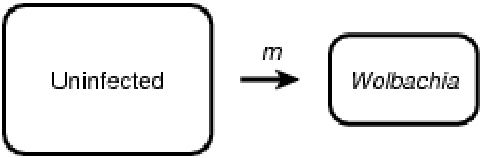
\includegraphics{uninfected_mainland.pdf}

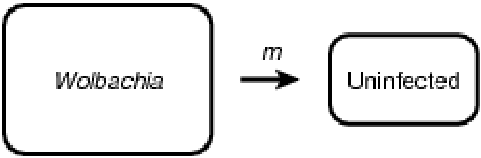
\includegraphics{infected_mainland.pdf}
\phantomsection\label{index:module-wspec.analytical}\index{wspec.analytical (module)}\phantomsection\label{index:module-analytical}\index{analytical (module)}\index{dynamics\_IM() (in module wspec.analytical)}

\begin{fulllineitems}
\phantomsection\label{index:wspec.analytical.dynamics_IM}\pysiglinewithargsret{\code{wspec.analytical.}\bfcode{dynamics\_IM}}{\emph{f}, \emph{ci}, \emph{m}, \emph{t}, \emph{x}}{}
Infection dynamics of Wolbachia for the scenario with an infected 
mainland (IM), iterative map.
\begin{description}
\item[{Args:}] \leavevmode\begin{description}
\item[{f: float in interval {[}0, 1{]}}] \leavevmode
fecundity reduction in infected females

\item[{ci: float in interval {[}0, 1{]}}] \leavevmode
level of CI

\item[{m: float in interval {[}0, 1{]}}] \leavevmode
migration rate

\item[{t: float in interval {[}0, 1{]}}] \leavevmode
transmission rate of Wolbachia

\item[{x: float in interval {[}0, 1{]}}] \leavevmode
infection frequency of Wolbachia

\end{description}

\item[{Returns:}] \leavevmode\begin{description}
\item[{out: float}] \leavevmode
infection frequency in the next generation

\end{description}

\end{description}

\end{fulllineitems}

\index{dynamics\_SP() (in module wspec.analytical)}

\begin{fulllineitems}
\phantomsection\label{index:wspec.analytical.dynamics_SP}\pysiglinewithargsret{\code{wspec.analytical.}\bfcode{dynamics\_SP}}{\emph{f}, \emph{ci}, \emph{t}, \emph{x}}{}
Infection dynamics of Wolbachia in a single host population (SP), 
iterative map returns the infection frequency in the next
generation.
\begin{description}
\item[{Args:}] \leavevmode\begin{description}
\item[{f: float in interval {[}0, 1{]}}] \leavevmode
fecundity reduction in infected females

\item[{ci: float in interval {[}0, 1{]}}] \leavevmode
level of CI

\item[{t: float in interval {[}0, 1{]}}] \leavevmode
transmission rate of Wolbachia

\item[{x: float in interval {[}0, 1{]}}] \leavevmode
infection frequency of Wolbachia

\end{description}

\item[{Returns:}] \leavevmode\begin{description}
\item[{out: float}] \leavevmode
infection frequency in the next generation

\end{description}

\end{description}

\end{fulllineitems}

\index{dynamics\_UM() (in module wspec.analytical)}

\begin{fulllineitems}
\phantomsection\label{index:wspec.analytical.dynamics_UM}\pysiglinewithargsret{\code{wspec.analytical.}\bfcode{dynamics\_UM}}{\emph{f}, \emph{ci}, \emph{m}, \emph{t}, \emph{x}}{}
Infection dynamics of Wolbachia for the scenario with an 
uninfected mainland (UM), iterative map returns the infection 
frequency in the next generation.
\begin{description}
\item[{Args:}] \leavevmode\begin{description}
\item[{f: float in interval {[}0, 1{]}}] \leavevmode
fecundity reduction in infected females

\item[{ci: float in interval {[}0, 1{]}}] \leavevmode
level of CI

\item[{m: float in interval {[}0, 1{]}}] \leavevmode
migration rate

\item[{t: float in interval {[}0, 1{]}}] \leavevmode
transmission rate of Wolbachia

\item[{x: float in interval {[}0, 1{]}}] \leavevmode
infection frequency of Wolbachia

\end{description}

\item[{Returns:}] \leavevmode\begin{description}
\item[{out: float}] \leavevmode
infection frequency in the next generation

\end{description}

\end{description}

\end{fulllineitems}

\index{fix1\_IM() (in module wspec.analytical)}

\begin{fulllineitems}
\phantomsection\label{index:wspec.analytical.fix1_IM}\pysiglinewithargsret{\code{wspec.analytical.}\bfcode{fix1\_IM}}{\emph{f}, \emph{ci}, \emph{m}, \emph{t}}{}
Fixpoint $x_1^{\ast}$ for the scenario with an infected mainland (IM).
\begin{description}
\item[{Args:}] \leavevmode\begin{description}
\item[{f: float in interval {[}0, 1{]}}] \leavevmode
fecundity reduction in infected females

\item[{ci: float in interval {[}0, 1{]}}] \leavevmode
level of CI

\item[{m: float in interval {[}0, 1{]}}] \leavevmode
migration rate

\item[{t: float in interval {[}0, 1{]}}] \leavevmode
transmission rate of Wolbachia

\end{description}

\item[{Returns:}] \leavevmode\begin{description}
\item[{out: float}] \leavevmode
critical migration rate

\end{description}

\end{description}

\end{fulllineitems}

\index{fix1\_SP() (in module wspec.analytical)}

\begin{fulllineitems}
\phantomsection\label{index:wspec.analytical.fix1_SP}\pysiglinewithargsret{\code{wspec.analytical.}\bfcode{fix1\_SP}}{\emph{f}, \emph{ci}, \emph{t}}{}
Infection frequency fixpoint $x_1^{\ast}$ for a single host population (SP).
\begin{description}
\item[{Args:}] \leavevmode\begin{description}
\item[{f: float in interval {[}0, 1{]}}] \leavevmode
fecundity reduction in infected females

\item[{ci: float in interval {[}0, 1{]}}] \leavevmode
level of CI

\item[{t: float in interval {[}0, 1{]}}] \leavevmode
transmission rate of Wolbachia

\end{description}

\item[{Returns:}] \leavevmode\begin{description}
\item[{out: float}] \leavevmode
equilibrium frequency of Wolbachia

\end{description}

\end{description}

\end{fulllineitems}

\index{fix1\_UM() (in module wspec.analytical)}

\begin{fulllineitems}
\phantomsection\label{index:wspec.analytical.fix1_UM}\pysiglinewithargsret{\code{wspec.analytical.}\bfcode{fix1\_UM}}{\emph{f}, \emph{ci}, \emph{m}, \emph{t}}{}
Fixpoint $x_1^{\ast}$ for the scenario with an uninfected mainland (UM).
\begin{description}
\item[{Args:}] \leavevmode\begin{description}
\item[{f: float in interval {[}0, 1{]}}] \leavevmode
fecundity reduction in infected females

\item[{ci: float in interval {[}0, 1{]}}] \leavevmode
level of CI

\item[{m: float in interval {[}0, 1{]}}] \leavevmode
migration rate

\item[{t: float in interval {[}0, 1{]}}] \leavevmode
transmission rate of Wolbachia

\end{description}

\item[{Returns:}] \leavevmode\begin{description}
\item[{out: float}] \leavevmode
equilibrium frequency of Wolbachia

\end{description}

\end{description}

\end{fulllineitems}

\index{fix2\_IM() (in module wspec.analytical)}

\begin{fulllineitems}
\phantomsection\label{index:wspec.analytical.fix2_IM}\pysiglinewithargsret{\code{wspec.analytical.}\bfcode{fix2\_IM}}{\emph{f}, \emph{ci}, \emph{m}, \emph{t}}{}
Fixpoint $x_2^{\ast}$ for the scenario with an infected mainland (IM).
\begin{description}
\item[{Args:}] \leavevmode\begin{description}
\item[{f: float in interval {[}0, 1{]}}] \leavevmode
fecundity reduction in infected females

\item[{ci: float in interval {[}0, 1{]}}] \leavevmode
level of CI

\item[{m: float in interval {[}0, 1{]}}] \leavevmode
migration rate

\item[{t: float in interval {[}0, 1{]}}] \leavevmode
transmission rate of Wolbachia

\end{description}

\item[{Returns:}] \leavevmode\begin{description}
\item[{out: float}] \leavevmode
critical migration rate

\end{description}

\end{description}

\end{fulllineitems}

\index{fix2\_SP() (in module wspec.analytical)}

\begin{fulllineitems}
\phantomsection\label{index:wspec.analytical.fix2_SP}\pysiglinewithargsret{\code{wspec.analytical.}\bfcode{fix2\_SP}}{\emph{f}, \emph{ci}, \emph{t}}{}
Infection frequency fixpoint $x_2^{\ast}$ for a single host population (SP).
\begin{description}
\item[{Args:}] \leavevmode\begin{description}
\item[{f: float in interval {[}0, 1{]}}] \leavevmode
fecundity reduction in infected females

\item[{ci: float in interval {[}0, 1{]}}] \leavevmode
level of CI

\item[{t: float in interval {[}0, 1{]}}] \leavevmode
transmission rate of Wolbachia

\end{description}

\item[{Returns:}] \leavevmode\begin{description}
\item[{out: float}] \leavevmode
equilibrium frequency of Wolbachia

\end{description}

\end{description}

\end{fulllineitems}

\index{fix2\_UM() (in module wspec.analytical)}

\begin{fulllineitems}
\phantomsection\label{index:wspec.analytical.fix2_UM}\pysiglinewithargsret{\code{wspec.analytical.}\bfcode{fix2\_UM}}{\emph{f}, \emph{ci}, \emph{m}, \emph{t}}{}
Fixpoint $x_2^{\ast}$ for the scenario with an uninfected mainland (UM).
\begin{description}
\item[{Args:}] \leavevmode\begin{description}
\item[{f: float in interval {[}0, 1{]}}] \leavevmode
fecundity reduction in infected females

\item[{ci: float in interval {[}0, 1{]}}] \leavevmode
level of CI

\item[{m: float in interval {[}0, 1{]}}] \leavevmode
migration rate

\item[{t: float in interval {[}0, 1{]}}] \leavevmode
transmission rate of Wolbachia

\end{description}

\item[{Returns:}] \leavevmode\begin{description}
\item[{out: float}] \leavevmode
equilibrium frequency of Wolbachia

\end{description}

\end{description}

\end{fulllineitems}

\index{fix3\_IM() (in module wspec.analytical)}

\begin{fulllineitems}
\phantomsection\label{index:wspec.analytical.fix3_IM}\pysiglinewithargsret{\code{wspec.analytical.}\bfcode{fix3\_IM}}{\emph{f}, \emph{ci}, \emph{m}, \emph{t}}{}
Fixpoint $x_3^{\ast}$ for the scenario with an infected mainland (IM).
\begin{description}
\item[{Args:}] \leavevmode\begin{description}
\item[{f: float in interval {[}0, 1{]}}] \leavevmode
fecundity reduction in infected females

\item[{ci: float in interval {[}0, 1{]}}] \leavevmode
level of CI

\item[{m: float in interval {[}0, 1{]}}] \leavevmode
migration rate

\item[{t: float in interval {[}0, 1{]}}] \leavevmode
transmission rate of Wolbachia

\end{description}

\item[{Returns:}] \leavevmode\begin{description}
\item[{out: float}] \leavevmode
critical migration rate

\end{description}

\end{description}

\end{fulllineitems}

\index{fix3\_SP() (in module wspec.analytical)}

\begin{fulllineitems}
\phantomsection\label{index:wspec.analytical.fix3_SP}\pysiglinewithargsret{\code{wspec.analytical.}\bfcode{fix3\_SP}}{\emph{f}, \emph{ci}, \emph{t}}{}
Infection frequency fixpoint $x_3^{\ast}$ for a single host population (SP).
\begin{description}
\item[{Args:}] \leavevmode\begin{description}
\item[{f: float in interval {[}0, 1{]}}] \leavevmode
fecundity reduction in infected females

\item[{ci: float in interval {[}0, 1{]}}] \leavevmode
level of CI

\item[{t: float in interval {[}0, 1{]}}] \leavevmode
transmission rate of Wolbachia

\end{description}

\item[{Returns:}] \leavevmode\begin{description}
\item[{out: float}] \leavevmode
equilibrium frequency of Wolbachia

\end{description}

\end{description}

\end{fulllineitems}

\index{fix3\_UM() (in module wspec.analytical)}

\begin{fulllineitems}
\phantomsection\label{index:wspec.analytical.fix3_UM}\pysiglinewithargsret{\code{wspec.analytical.}\bfcode{fix3\_UM}}{\emph{f}, \emph{ci}, \emph{m}, \emph{t}}{}
Fixpoint $x_3^{\ast}$ for the scenario with an uninfected mainland (UM).
\begin{description}
\item[{Args:}] \leavevmode\begin{description}
\item[{f: float in interval {[}0, 1{]}}] \leavevmode
fecundity reduction in infected females

\item[{ci: float in interval {[}0, 1{]}}] \leavevmode
level of CI

\item[{m: float in interval {[}0, 1{]}}] \leavevmode
migration rate

\item[{t: float in interval {[}0, 1{]}}] \leavevmode
transmission rate of Wolbachia

\end{description}

\item[{Returns:}] \leavevmode\begin{description}
\item[{out: float}] \leavevmode
equilibrium frequency of Wolbachia

\end{description}

\end{description}

\end{fulllineitems}

\index{fix\_SP() (in module wspec.analytical)}

\begin{fulllineitems}
\phantomsection\label{index:wspec.analytical.fix_SP}\pysiglinewithargsret{\code{wspec.analytical.}\bfcode{fix\_SP}}{\emph{f}, \emph{ci}, \emph{t}}{}
Infection frequency fixpoints for a single host population (SP).
\begin{description}
\item[{Args:}] \leavevmode\begin{description}
\item[{f: float in interval {[}0, 1{]}}] \leavevmode
fecundity reduction in infected females

\item[{ci: float in interval {[}0, 1{]}}] \leavevmode
level of CI

\item[{t: float in interval {[}0, 1{]}}] \leavevmode
transmission rate of Wolbachia

\end{description}

\item[{Returns:}] \leavevmode\begin{description}
\item[{out: tuple of three floats}] \leavevmode
equilibrium frequencies $x_1^{\ast}$, $x_2^{\ast}$, and $x_3^{\ast}$ of Wolbachia

\end{description}

\end{description}

\end{fulllineitems}

\index{fix\_UM() (in module wspec.analytical)}

\begin{fulllineitems}
\phantomsection\label{index:wspec.analytical.fix_UM}\pysiglinewithargsret{\code{wspec.analytical.}\bfcode{fix\_UM}}{\emph{f}, \emph{ci}, \emph{m}, \emph{t}}{}
Infection frequency fixpoints for the scenario with an infected 
mainland (IM).
\begin{description}
\item[{Args:}] \leavevmode\begin{description}
\item[{f: float in interval {[}0, 1{]}}] \leavevmode
fecundity reduction in infected females

\item[{ci: float in interval {[}0, 1{]}}] \leavevmode
level of CI

\item[{m: float in interval {[}0, 1{]}}] \leavevmode
migration rate

\item[{t: float in interval {[}0, 1{]}}] \leavevmode
transmission rate of Wolbachia

\end{description}

\item[{Returns:}] \leavevmode\begin{description}
\item[{out: tuple of three floats}] \leavevmode
equilibrium frequencies $x_1^{\ast}$, $x_2^{\ast}$, and $x_3^{\ast}$ of Wolbachia

\end{description}

\end{description}

\end{fulllineitems}

\index{gff\_DS() (in module wspec.analytical)}

\begin{fulllineitems}
\phantomsection\label{index:wspec.analytical.gff_DS}\pysiglinewithargsret{\code{wspec.analytical.}\bfcode{gff\_DS}}{\emph{m}, \emph{s}}{}
Gene flow factor (gff) for the case of divergent selection (DS).
Residents have a viability advantage of \emph{s} over migrants, 
equivalent to migrants having a viability cost of $\frac{s}{1+s}$.
Derived from fitness graph for the reproductive value of a migrant.
\begin{description}
\item[{Args:}] \leavevmode\begin{description}
\item[{m: float in interval {[}0, 1{]}}] \leavevmode
migration rate

\item[{s: positive float}] \leavevmode
selection coefficient

\end{description}

\item[{Returns:}] \leavevmode\begin{description}
\item[{out: float}] \leavevmode
gene flow factor

\end{description}

\end{description}

\end{fulllineitems}

\index{lcrit\_SP() (in module wspec.analytical)}

\begin{fulllineitems}
\phantomsection\label{index:wspec.analytical.lcrit_SP}\pysiglinewithargsret{\code{wspec.analytical.}\bfcode{lcrit\_SP}}{\emph{f}, \emph{t}}{}
Critical CI level (lcrit) for a single host population (SP).
\begin{description}
\item[{Args:}] \leavevmode\begin{description}
\item[{f: float in interval {[}0, 1{]}}] \leavevmode
fecundity reduction in infected females

\item[{t: float in interval {[}0, 1{]}}] \leavevmode
transmission rate of Wolbachia

\end{description}

\item[{Returns:}] \leavevmode\begin{description}
\item[{out: float}] \leavevmode
critical CI level

\end{description}

\end{description}

\end{fulllineitems}

\index{lcrit\_UM() (in module wspec.analytical)}

\begin{fulllineitems}
\phantomsection\label{index:wspec.analytical.lcrit_UM}\pysiglinewithargsret{\code{wspec.analytical.}\bfcode{lcrit\_UM}}{\emph{f}, \emph{m}, \emph{t}}{}
Critical CI level (lcrit) for the scenario with an uninfected 
mainland (UM).
\begin{description}
\item[{Args:}] \leavevmode\begin{description}
\item[{f: float in interval {[}0, 1{]}}] \leavevmode
fecundity reduction in infected females

\item[{m: float in interval {[}0, 1{]}}] \leavevmode
migration rate

\item[{t: float in interval {[}0, 1{]}}] \leavevmode
transmission rate of Wolbachia

\end{description}

\item[{Returns:}] \leavevmode\begin{description}
\item[{out: float}] \leavevmode
critical CI level

\end{description}

\end{description}

\end{fulllineitems}

\index{mcrit\_IM() (in module wspec.analytical)}

\begin{fulllineitems}
\phantomsection\label{index:wspec.analytical.mcrit_IM}\pysiglinewithargsret{\code{wspec.analytical.}\bfcode{mcrit\_IM}}{\emph{f}, \emph{ci}, \emph{t}}{}
Critical migration rate (mcrit) for the scenario with an infected 
mainland (IM).
\begin{description}
\item[{Args:}] \leavevmode\begin{description}
\item[{f: float in interval {[}0, 1{]}}] \leavevmode
fecundity reduction in infected females

\item[{ci: float in interval {[}0, 1{]}}] \leavevmode
level of CI

\item[{t: float in interval {[}0, 1{]}}] \leavevmode
transmission rate of Wolbachia

\end{description}

\item[{Returns:}] \leavevmode\begin{description}
\item[{out: float}] \leavevmode
critical migration rate

\end{description}

\end{description}

\end{fulllineitems}

\index{mcrit\_IMA() (in module wspec.analytical)}

\begin{fulllineitems}
\phantomsection\label{index:wspec.analytical.mcrit_IMA}\pysiglinewithargsret{\code{wspec.analytical.}\bfcode{mcrit\_IMA}}{\emph{f}, \emph{ci}, \emph{s}, \emph{t}}{}
Critical migration rate (mcrit) for the scenario with an infected 
mainland (IM) with local host adaptation (A).
\begin{description}
\item[{Args:}] \leavevmode\begin{description}
\item[{f: float in interval {[}0, 1{]}}] \leavevmode
fecundity reduction in infected females

\item[{ci: float in interval {[}0, 1{]}}] \leavevmode
level of CI

\item[{s: positive float}] \leavevmode
selection coefficient

\item[{t: float in interval {[}0, 1{]}}] \leavevmode
transmission rate of Wolbachia

\end{description}

\item[{Returns:}] \leavevmode\begin{description}
\item[{out: float}] \leavevmode
critical migration rate

\end{description}

\end{description}

\end{fulllineitems}

\index{mcrit\_UM() (in module wspec.analytical)}

\begin{fulllineitems}
\phantomsection\label{index:wspec.analytical.mcrit_UM}\pysiglinewithargsret{\code{wspec.analytical.}\bfcode{mcrit\_UM}}{\emph{f}, \emph{ci}, \emph{t}}{}
Critical migration rate (mcrit) for the scenario with an uninfected 
mainland (UM).
\begin{description}
\item[{Args:}] \leavevmode\begin{description}
\item[{f: float in interval {[}0, 1{]}}] \leavevmode
fecundity reduction in infected females

\item[{ci: float in interval {[}0, 1{]}}] \leavevmode
level of CI

\item[{t: float in interval {[}0, 1{]}}] \leavevmode
transmission rate of Wolbachia

\end{description}

\item[{Returns:}] \leavevmode\begin{description}
\item[{out: float}] \leavevmode
critical migration rate

\end{description}

\end{description}

\end{fulllineitems}

\index{mcrit\_UMA() (in module wspec.analytical)}

\begin{fulllineitems}
\phantomsection\label{index:wspec.analytical.mcrit_UMA}\pysiglinewithargsret{\code{wspec.analytical.}\bfcode{mcrit\_UMA}}{\emph{f}, \emph{ci}, \emph{s}, \emph{t}}{}
Critical migration rate (mcrit) for the scenario with an uninfected 
mainland (UM) with local host adaptation (A).
\begin{description}
\item[{Args:}] \leavevmode\begin{description}
\item[{f: float in interval {[}0, 1{]}}] \leavevmode
fecundity reduction in infected females

\item[{ci: float in interval {[}0, 1{]}}] \leavevmode
level of CI

\item[{s: positive float}] \leavevmode
selection coefficient

\item[{t: float in interval {[}0, 1{]}}] \leavevmode
transmission rate of Wolbachia

\end{description}

\item[{Returns:}] \leavevmode\begin{description}
\item[{out: float}] \leavevmode
critical migration rate

\end{description}

\end{description}

\end{fulllineitems}

\index{meff\_DS() (in module wspec.analytical)}

\begin{fulllineitems}
\phantomsection\label{index:wspec.analytical.meff_DS}\pysiglinewithargsret{\code{wspec.analytical.}\bfcode{meff\_DS}}{\emph{m}, \emph{s}}{}
Effective migration rate (meff) for the case of divergent selection 
(DS). Residents have a viability advantage of \emph{s} over migrants, 
equivalent to migrants having a viability cost of $\frac{s}{1+s}$.
Derived from fitness graph for the reproductive value of a migrant.
\begin{description}
\item[{Args:}] \leavevmode\begin{description}
\item[{m: float in interval {[}0, 1{]}}] \leavevmode
migration rate

\item[{s: positive float}] \leavevmode
selection coefficient

\end{description}

\item[{Returns:}] \leavevmode\begin{description}
\item[{out: float}] \leavevmode
effective migration rate

\end{description}

\end{description}

\end{fulllineitems}

\index{prcrit() (in module wspec.analytical)}

\begin{fulllineitems}
\phantomsection\label{index:wspec.analytical.prcrit}\pysiglinewithargsret{\code{wspec.analytical.}\bfcode{prcrit}}{\emph{ci}, \emph{q}, \emph{s}}{}
Minimal rejection probability (pr) of a mutant allele at the locus 
for female mating preference to spread in an uninfected island 
receiving migration from an infected mainland.
\begin{description}
\item[{Args:}] \leavevmode\begin{description}
\item[{ci: float in interval {[}0, 1{]}}] \leavevmode
level of CI

\item[{q: float in interval {[}0, 1{]}}] \leavevmode
transition probability to a new mating round

\item[{s: positive float}] \leavevmode
selection coefficient

\end{description}

\item[{Returns:}] \leavevmode\begin{description}
\item[{out: float}] \leavevmode
minimal rejection probability

\end{description}

\end{description}

\end{fulllineitems}

\index{reproval\_DS() (in module wspec.analytical)}

\begin{fulllineitems}
\phantomsection\label{index:wspec.analytical.reproval_DS}\pysiglinewithargsret{\code{wspec.analytical.}\bfcode{reproval\_DS}}{\emph{s}}{}
Reproductive value of a migrant for the case of divergent 
selection (DS). Residents have a viability advantage of \emph{s} over 
migrants, equivalent to migrants having a viability cost of 
$\frac{s}{1+s}$. Derived from fitness graph.
\begin{description}
\item[{Args:}] \leavevmode\begin{description}
\item[{s: positive float}] \leavevmode
selection coefficient

\end{description}

\item[{Returns:}] \leavevmode\begin{description}
\item[{out: float}] \leavevmode
reproductive value

\end{description}

\end{description}

\end{fulllineitems}

\index{reproval\_FUHETCL() (in module wspec.analytical)}

\begin{fulllineitems}
\phantomsection\label{index:wspec.analytical.reproval_FUHETCL}\pysiglinewithargsret{\code{wspec.analytical.}\bfcode{reproval\_FUHETCL}}{\emph{f}, \emph{ci}, \emph{t}}{}
Reproductive value of an uninfected female (FU) in a 
heterogenous host population (HET), \emph{per class} (CL) reproductive 
value (as opposed to \emph{per capita}). Derived from fitness graph.
\begin{description}
\item[{Args:}] \leavevmode\begin{description}
\item[{f: float in interval {[}0, 1{]}}] \leavevmode
fecundity reduction in infected females

\item[{ci: float in interval {[}0, 1{]}}] \leavevmode
level of CI

\item[{t: float in interval {[}0, 1{]}}] \leavevmode
transmission rate of Wolbachia

\end{description}

\item[{Returns:}] \leavevmode\begin{description}
\item[{out: float}] \leavevmode
reproductive value

\end{description}

\end{description}

\end{fulllineitems}

\index{reproval\_FUHETCP() (in module wspec.analytical)}

\begin{fulllineitems}
\phantomsection\label{index:wspec.analytical.reproval_FUHETCP}\pysiglinewithargsret{\code{wspec.analytical.}\bfcode{reproval\_FUHETCP}}{\emph{f}, \emph{ci}, \emph{t}}{}
Reproductive value of an uninfected female (FU) in a 
heterogenous host population (HET), \emph{per capita} (CP) reproductive 
value (as opposed to \emph{per class}). Derived from fitness graph.
\begin{description}
\item[{Args:}] \leavevmode\begin{description}
\item[{f: float in interval {[}0, 1{]}}] \leavevmode
fecundity reduction in infected females

\item[{ci: float in interval {[}0, 1{]}}] \leavevmode
level of CI

\item[{t: float in interval {[}0, 1{]}}] \leavevmode
transmission rate of Wolbachia

\end{description}

\item[{Returns:}] \leavevmode\begin{description}
\item[{out: float}] \leavevmode
reproductive value

\end{description}

\end{description}

\end{fulllineitems}

\index{reproval\_FUHOMW() (in module wspec.analytical)}

\begin{fulllineitems}
\phantomsection\label{index:wspec.analytical.reproval_FUHOMW}\pysiglinewithargsret{\code{wspec.analytical.}\bfcode{reproval\_FUHOMW}}{\emph{f}, \emph{ci}}{}
Reproductive value of an uninfected female migrant (FU) in a 
homogenous Wolbachia infected population (HOMW). This applies to 
the case of perfect Wolbachia transmission, $t=1$. Derived from 
fitness graph:
\begin{description}
\item[{Args:}] \leavevmode\begin{description}
\item[{f: float in interval {[}0, 1{]}}] \leavevmode
fecundity reduction in infected females

\item[{ci: float in interval {[}0, 1{]}}] \leavevmode
level of CI

\end{description}

\item[{Returns:}] \leavevmode\begin{description}
\item[{out: float}] \leavevmode
reproductive value

\end{description}

\end{description}

\end{fulllineitems}

\index{reproval\_FWHETCL() (in module wspec.analytical)}

\begin{fulllineitems}
\phantomsection\label{index:wspec.analytical.reproval_FWHETCL}\pysiglinewithargsret{\code{wspec.analytical.}\bfcode{reproval\_FWHETCL}}{\emph{f}, \emph{ci}, \emph{t}}{}
Reproductive value of an infected female (FW) in a heterogenous 
host population (HET), \emph{per class} (CL) reproductive value (as 
opposed to \emph{per capita}). Derived from fitness graph.
\begin{description}
\item[{Args:}] \leavevmode\begin{description}
\item[{f: float in interval {[}0, 1{]}}] \leavevmode
fecundity reduction in infected females

\item[{ci: float in interval {[}0, 1{]}}] \leavevmode
level of CI

\item[{t: float in interval {[}0, 1{]}}] \leavevmode
transmission rate of Wolbachia

\end{description}

\item[{Returns:}] \leavevmode\begin{description}
\item[{out: float}] \leavevmode
reproductive value

\end{description}

\end{description}

\end{fulllineitems}

\index{reproval\_FWHETCP() (in module wspec.analytical)}

\begin{fulllineitems}
\phantomsection\label{index:wspec.analytical.reproval_FWHETCP}\pysiglinewithargsret{\code{wspec.analytical.}\bfcode{reproval\_FWHETCP}}{\emph{f}, \emph{ci}, \emph{t}}{}
Reproductive value of a Wolbachia infected female (FW) in a 
heterogenous host population (HET), \emph{per capita} (CP) reproductive 
value (as opposed to \emph{per class}). Derived from fitness graph.
\begin{description}
\item[{Args:}] \leavevmode\begin{description}
\item[{f: float in interval {[}0, 1{]}}] \leavevmode
fecundity reduction in infected females

\item[{ci: float in interval {[}0, 1{]}}] \leavevmode
level of CI

\item[{t: float in interval {[}0, 1{]}}] \leavevmode
transmission rate of Wolbachia

\end{description}

\item[{Returns:}] \leavevmode\begin{description}
\item[{out: float}] \leavevmode
reproductive value

\end{description}

\end{description}

\end{fulllineitems}

\index{reproval\_FWHOMU() (in module wspec.analytical)}

\begin{fulllineitems}
\phantomsection\label{index:wspec.analytical.reproval_FWHOMU}\pysiglinewithargsret{\code{wspec.analytical.}\bfcode{reproval\_FWHOMU}}{\emph{f}, \emph{ci}, \emph{t}}{}
Reproductive value of a Wolbachia infected female migrant (FW)
in a homogenous uninfected population (HOMU). Derived from fitness 
graph.
\begin{description}
\item[{Args:}] \leavevmode\begin{description}
\item[{f: float in interval {[}0, 1{]}}] \leavevmode
fecundity reduction in infected females

\item[{ci: float in interval {[}0, 1{]}}] \leavevmode
level of CI

\item[{t: float in interval {[}0, 1{]}}] \leavevmode
transmission rate of Wolbachia

\end{description}

\item[{Returns:}] \leavevmode\begin{description}
\item[{out: float}] \leavevmode
reproductive value

\end{description}

\end{description}

\end{fulllineitems}

\index{reproval\_IPHOMU() (in module wspec.analytical)}

\begin{fulllineitems}
\phantomsection\label{index:wspec.analytical.reproval_IPHOMU}\pysiglinewithargsret{\code{wspec.analytical.}\bfcode{reproval\_IPHOMU}}{\emph{f}, \emph{ci}, \emph{t}}{}
Average reproductive value of a migrant from an infected 
population (IP), i.e. where the Wolbachia infection is at a stable 
frequency below 1 due to imperfect transmission, in a homogenous 
uninfected population (HOU). Averaged over sexes (F/M) and 
cytotypes (U/W). Derived from fitness graph.
\begin{description}
\item[{Args:}] \leavevmode\begin{description}
\item[{f: float in interval {[}0, 1{]}}] \leavevmode
fecundity reduction in infected females

\item[{ci: float in interval {[}0, 1{]}}] \leavevmode
level of CI

\item[{t: float in interval {[}0, 1{]}}] \leavevmode
transmission rate of Wolbachia

\end{description}

\item[{Returns:}] \leavevmode\begin{description}
\item[{out: float}] \leavevmode
reproductive value

\end{description}

\end{description}

\end{fulllineitems}

\index{reproval\_MUHETCL() (in module wspec.analytical)}

\begin{fulllineitems}
\phantomsection\label{index:wspec.analytical.reproval_MUHETCL}\pysiglinewithargsret{\code{wspec.analytical.}\bfcode{reproval\_MUHETCL}}{\emph{f}, \emph{ci}, \emph{t}}{}
Reproductive value of an uninfected male (MU) in a heterogenous 
host population (HET), \emph{per class} (CL) reproductive value (as 
opposed to \emph{per capita}). Derived from fitness graph.
\begin{description}
\item[{Args:}] \leavevmode\begin{description}
\item[{f: float in interval {[}0, 1{]}}] \leavevmode
fecundity reduction in infected females

\item[{ci: float in interval {[}0, 1{]}}] \leavevmode
level of CI

\item[{t: float in interval {[}0, 1{]}}] \leavevmode
transmission rate of Wolbachia

\end{description}

\item[{Returns:}] \leavevmode\begin{description}
\item[{out: float}] \leavevmode
reproductive value

\end{description}

\end{description}

\end{fulllineitems}

\index{reproval\_MUHETCP() (in module wspec.analytical)}

\begin{fulllineitems}
\phantomsection\label{index:wspec.analytical.reproval_MUHETCP}\pysiglinewithargsret{\code{wspec.analytical.}\bfcode{reproval\_MUHETCP}}{\emph{f}, \emph{ci}, \emph{t}}{}
Reproductive value of an uninfected male (MU) in a heterogenous 
host population (HET), \emph{per capita} (CP) reproductive value (as 
opposed to \emph{per class}). Derived from fitness graph.
\begin{description}
\item[{Args:}] \leavevmode\begin{description}
\item[{f: float in interval {[}0, 1{]}}] \leavevmode
fecundity reduction in infected females

\item[{ci: float in interval {[}0, 1{]}}] \leavevmode
level of CI

\item[{t: float in interval {[}0, 1{]}}] \leavevmode
transmission rate of Wolbachia

\end{description}

\item[{Returns:}] \leavevmode\begin{description}
\item[{out: float}] \leavevmode
reproductive value

\end{description}

\end{description}

\end{fulllineitems}

\index{reproval\_MUHOMW() (in module wspec.analytical)}

\begin{fulllineitems}
\phantomsection\label{index:wspec.analytical.reproval_MUHOMW}\pysiglinewithargsret{\code{wspec.analytical.}\bfcode{reproval\_MUHOMW}}{\emph{f}, \emph{ci}}{}
Reproductive value of an uninfected male migrant (MU) in a 
homogenous Wolbachia infected population (HOMW). This applies to 
the case of perfect Wolbachia transmission, t=1.
Derived from fitness graph.
\begin{description}
\item[{Args:}] \leavevmode\begin{description}
\item[{f: float in interval {[}0, 1{]}}] \leavevmode
fecundity reduction in infected females

\item[{ci: float in interval {[}0, 1{]}}] \leavevmode
level of CI

\end{description}

\item[{Returns:}] \leavevmode\begin{description}
\item[{out: float}] \leavevmode
reproductive value

\end{description}

\end{description}

\end{fulllineitems}

\index{reproval\_MWHETCL() (in module wspec.analytical)}

\begin{fulllineitems}
\phantomsection\label{index:wspec.analytical.reproval_MWHETCL}\pysiglinewithargsret{\code{wspec.analytical.}\bfcode{reproval\_MWHETCL}}{\emph{f}, \emph{ci}, \emph{t}}{}
Reproductive value of an infected male (MW) in a heterogenous 
host population (HET), \emph{per class} (CL) reproductive value (as 
opposed to \emph{per capita}). Derived from fitness graph.
\begin{description}
\item[{Args:}] \leavevmode\begin{description}
\item[{f: float in interval {[}0, 1{]}}] \leavevmode
fecundity reduction in infected females

\item[{ci: float in interval {[}0, 1{]}}] \leavevmode
level of CI

\item[{t: float in interval {[}0, 1{]}}] \leavevmode
transmission rate of Wolbachia

\end{description}

\item[{Returns:}] \leavevmode\begin{description}
\item[{out: float}] \leavevmode
reproductive value

\end{description}

\end{description}

\end{fulllineitems}

\index{reproval\_MWHETCP() (in module wspec.analytical)}

\begin{fulllineitems}
\phantomsection\label{index:wspec.analytical.reproval_MWHETCP}\pysiglinewithargsret{\code{wspec.analytical.}\bfcode{reproval\_MWHETCP}}{\emph{f}, \emph{ci}, \emph{t}}{}
Reproductive value of a Wolbachia infected male (MW) in a 
heterogenous host population (HET), \emph{per capita} (CP) reproductive 
value (as opposed to \emph{per class}). Derived from fitness graph.
\begin{description}
\item[{Args:}] \leavevmode\begin{description}
\item[{f: float in interval {[}0, 1{]}}] \leavevmode
fecundity reduction in infected females

\item[{ci: float in interval {[}0, 1{]}}] \leavevmode
level of CI

\item[{t: float in interval {[}0, 1{]}}] \leavevmode
transmission rate of Wolbachia

\end{description}

\item[{Returns:}] \leavevmode\begin{description}
\item[{out: float}] \leavevmode
reproductive value

\end{description}

\end{description}

\end{fulllineitems}

\index{reproval\_MWHOMU() (in module wspec.analytical)}

\begin{fulllineitems}
\phantomsection\label{index:wspec.analytical.reproval_MWHOMU}\pysiglinewithargsret{\code{wspec.analytical.}\bfcode{reproval\_MWHOMU}}{\emph{f}, \emph{ci}, \emph{t}}{}
Reproductive value of a Wolbachia infected male migrant (MW) 
in a homogenous uninfected population (HOMU). Derived from fitness 
graph.
\begin{description}
\item[{Args:}] \leavevmode\begin{description}
\item[{f: float in interval {[}0, 1{]}}] \leavevmode
fecundity reduction in infected females

\item[{ci: float in interval {[}0, 1{]}}] \leavevmode
level of CI

\item[{t: float in interval {[}0, 1{]}}] \leavevmode
transmission rate of Wolbachia

\end{description}

\item[{Returns:}] \leavevmode\begin{description}
\item[{out: float}] \leavevmode
reproductive value

\end{description}

\end{description}

\end{fulllineitems}

\index{reproval\_UHETCL() (in module wspec.analytical)}

\begin{fulllineitems}
\phantomsection\label{index:wspec.analytical.reproval_UHETCL}\pysiglinewithargsret{\code{wspec.analytical.}\bfcode{reproval\_UHETCL}}{\emph{f}, \emph{ci}, \emph{t}}{}
Average reproductive value of an uninfected host (U) in a 
heterogenous population (HET), \emph{per class} (CL) reproductive value 
(as opposed to \emph{per capita}). Derived from fitness graph. 
Averaged over the two sexes.
\begin{description}
\item[{Args:}] \leavevmode\begin{description}
\item[{f: float in interval {[}0, 1{]}}] \leavevmode
fecundity reduction in infected females

\item[{ci: float in interval {[}0, 1{]}}] \leavevmode
level of CI

\item[{t: float in interval {[}0, 1{]}}] \leavevmode
transmission rate of Wolbachia

\end{description}

\item[{Returns:}] \leavevmode\begin{description}
\item[{out: float}] \leavevmode
reproductive value

\end{description}

\end{description}

\end{fulllineitems}

\index{reproval\_UHETCP() (in module wspec.analytical)}

\begin{fulllineitems}
\phantomsection\label{index:wspec.analytical.reproval_UHETCP}\pysiglinewithargsret{\code{wspec.analytical.}\bfcode{reproval\_UHETCP}}{\emph{f}, \emph{ci}, \emph{t}}{}
Average reproductive value of an uninfected host (U) in a 
heterogenous population (HET), \emph{per capita} (CP) reproductive 
value (as opposed to \emph{per class}). Derived from fitness graph. 
Averaged over the two sexes.
\begin{description}
\item[{Args:}] \leavevmode\begin{description}
\item[{f: float in interval {[}0, 1{]}}] \leavevmode
fecundity reduction in infected females

\item[{ci: float in interval {[}0, 1{]}}] \leavevmode
level of CI

\item[{t: float in interval {[}0, 1{]}}] \leavevmode
transmission rate of Wolbachia

\end{description}

\item[{Returns:}] \leavevmode\begin{description}
\item[{out: float}] \leavevmode
reproductive value

\end{description}

\end{description}

\end{fulllineitems}

\index{reproval\_UHOMW() (in module wspec.analytical)}

\begin{fulllineitems}
\phantomsection\label{index:wspec.analytical.reproval_UHOMW}\pysiglinewithargsret{\code{wspec.analytical.}\bfcode{reproval\_UHOMW}}{\emph{f}, \emph{ci}}{}
Reproductive value of an uninfected migrant (U) in a a 
homogenous Wolbachia infected population (HOMW). This applies to 
the case of perfect Wolbachia transmission, t=1. Derived from 
fitness graph. Averaged over the two sexes.
\begin{description}
\item[{Args:}] \leavevmode\begin{description}
\item[{f: float in interval {[}0, 1{]}}] \leavevmode
fecundity reduction in infected females

\item[{ci: float in interval {[}0, 1{]}}] \leavevmode
level of CI

\end{description}

\item[{Returns:}] \leavevmode\begin{description}
\item[{out: float}] \leavevmode
reproductive value

\end{description}

\end{description}

\end{fulllineitems}

\index{reproval\_WHETCL() (in module wspec.analytical)}

\begin{fulllineitems}
\phantomsection\label{index:wspec.analytical.reproval_WHETCL}\pysiglinewithargsret{\code{wspec.analytical.}\bfcode{reproval\_WHETCL}}{\emph{f}, \emph{ci}, \emph{t}}{}
Reproductive value of an infected host (W) in a heterogenous host 
population (HET), \emph{per class} (CL) reproductive value (as opposed to \emph{per 
capita}). Derived from fitness graph.
\begin{description}
\item[{Args:}] \leavevmode\begin{description}
\item[{f: float in interval {[}0, 1{]}}] \leavevmode
fecundity reduction in infected females

\item[{ci: float in interval {[}0, 1{]}}] \leavevmode
level of CI

\item[{t: float in interval {[}0, 1{]}}] \leavevmode
transmission rate of Wolbachia

\end{description}

\item[{Returns:}] \leavevmode\begin{description}
\item[{out: float}] \leavevmode
reproductive value

\end{description}

\end{description}

\end{fulllineitems}

\index{reproval\_WHETCP() (in module wspec.analytical)}

\begin{fulllineitems}
\phantomsection\label{index:wspec.analytical.reproval_WHETCP}\pysiglinewithargsret{\code{wspec.analytical.}\bfcode{reproval\_WHETCP}}{\emph{f}, \emph{ci}, \emph{t}}{}
Average reproductive value of a Wolbachia infected host (W) in 
a heterogenous population (HET), \emph{per capita} (CP) reproductive 
value (as opposed to \emph{per class}). Derived from fitness graph. 
Averaged over the two sexes.
\begin{description}
\item[{Args:}] \leavevmode\begin{description}
\item[{f: float in interval {[}0, 1{]}}] \leavevmode
fecundity reduction in infected females

\item[{ci: float in interval {[}0, 1{]}}] \leavevmode
level of CI

\item[{t: float in interval {[}0, 1{]}}] \leavevmode
transmission rate of Wolbachia

\end{description}

\item[{Returns:}] \leavevmode\begin{description}
\item[{out: float}] \leavevmode
reproductive value

\end{description}

\end{description}

\end{fulllineitems}

\index{reproval\_WHOMU() (in module wspec.analytical)}

\begin{fulllineitems}
\phantomsection\label{index:wspec.analytical.reproval_WHOMU}\pysiglinewithargsret{\code{wspec.analytical.}\bfcode{reproval\_WHOMU}}{\emph{f}, \emph{ci}, \emph{t}}{}
Reproductive value of a Wolbachia infected migrant (W) in a 
homogenous uninfected population (HOU). Derived from fitness graph.
Averaged over the two sexes.
\begin{description}
\item[{Args:}] \leavevmode\begin{description}
\item[{f: float in interval {[}0, 1{]}}] \leavevmode
fecundity reduction in infected females

\item[{ci: float in interval {[}0, 1{]}}] \leavevmode
level of CI

\item[{t: float in interval {[}0, 1{]}}] \leavevmode
transmission rate of Wolbachia

\end{description}

\item[{Returns:}] \leavevmode\begin{description}
\item[{out: float}] \leavevmode
reproductive value

\end{description}

\end{description}

\end{fulllineitems}

\index{xPref() (in module wspec.analytical)}

\begin{fulllineitems}
\phantomsection\label{index:wspec.analytical.xPref}\pysiglinewithargsret{\code{wspec.analytical.}\bfcode{xPref}}{\emph{ci}, \emph{pr}, \emph{q}, \emph{s}}{}
Approximated equilibrium frequency of a mutant allele at the locus 
for female mating preference in an uninfected island receiving 
migration from an infected mainland.
\begin{description}
\item[{Args:}] \leavevmode\begin{description}
\item[{ci: float in interval {[}0, 1{]}}] \leavevmode
level of CI

\item[{pr: float in interval {[}0, 1{]}}] \leavevmode
rejection probability of mating preference mutant allele

\item[{q: float in interval {[}0, 1{]}}] \leavevmode
transition probability to a new mating round

\item[{s: positive float}] \leavevmode
selection coefficient

\end{description}

\item[{Returns:}] \leavevmode\begin{description}
\item[{out: float}] \leavevmode
equilibrium frequency of mutant preference allele

\end{description}

\end{description}

\end{fulllineitems}

\index{xTprefEQ() (in module wspec.analytical)}

\begin{fulllineitems}
\phantomsection\label{index:wspec.analytical.xTprefEQ}\pysiglinewithargsret{\code{wspec.analytical.}\bfcode{xTprefEQ}}{\emph{pr}, \emph{s}, \emph{xPref}}{}
Modified from Kirkpatrick (1982), equation (2).
\begin{description}
\item[{Args:}] \leavevmode\begin{description}
\item[{pr: float in interval {[}0, 1{]}}] \leavevmode
rejection probability of mating preference mutant allele

\item[{s: positive float}] \leavevmode
selection coefficient

\item[{xPref: float in interval {[}0, 1{]}}] \leavevmode
frequency of preference allele in Kirkpatrick's model

\end{description}

\item[{Returns:}] \leavevmode\begin{description}
\item[{out: float}] \leavevmode
equilibrium frequency of preferred trait

\end{description}

\end{description}

\end{fulllineitems}



\chapter{Indices and tables}
\label{index:indices-and-tables}\begin{itemize}
\item {} 
\emph{genindex}

\item {} 
\emph{modindex}

\item {} 
\emph{search}

\end{itemize}


\renewcommand{\indexname}{Python Module Index}
\begin{theindex}
\def\bigletter#1{{\Large\sffamily#1}\nopagebreak\vspace{1mm}}
\bigletter{a}
\item {\texttt{analytical}} \emph{(Unix)}, \pageref{index:module-analytical}
\indexspace
\bigletter{w}
\item {\texttt{wspec.analytical}}, \pageref{index:module-wspec.analytical}
\end{theindex}

\renewcommand{\indexname}{Index}
\printindex
\end{document}
